\section{Architecture}
\label{Arc}
\subsection{Overview}
Before introducing our SDN system architecture, we first present some basic terms in SDN system,.

\textbf{Data plane}: forwarding data and basic sensing functions.

\textbf{Control plane}: the protocols used to populate the forwarding tables of data plane elements.

\textbf{Management plane}: software services. network policy is defined in management plane, the control plane enforces the policy, and  the data plane executes it by forwarding data accordingly. (running applications)

\textbf{Southbound Interface (SI)}: The instruction set of the forwarding devices is defined by the southbound API, which is part of the southbound interface. Furthermore, the SI also defines the communication protocol between data plane and control plane elements. This protocol formalizes the way the control and data plane elements interact.

\textbf{Northbound Interface (NI)}: The middleware on control plane can offer an API to application developers. This API represents a northbound interface, i.e., a common interface for developing applications. Typically, a northbound interface make abstracts the low-level instruction sets used by southbound interfaces to program forwarding devices.


The architecture of {\sdn} is shown in Fig. \ref{Architecture}. 
The system is divided into three layers: data plane, 
control plane and management plane respectively.

\begin{figure}[htbp]
	\centering
	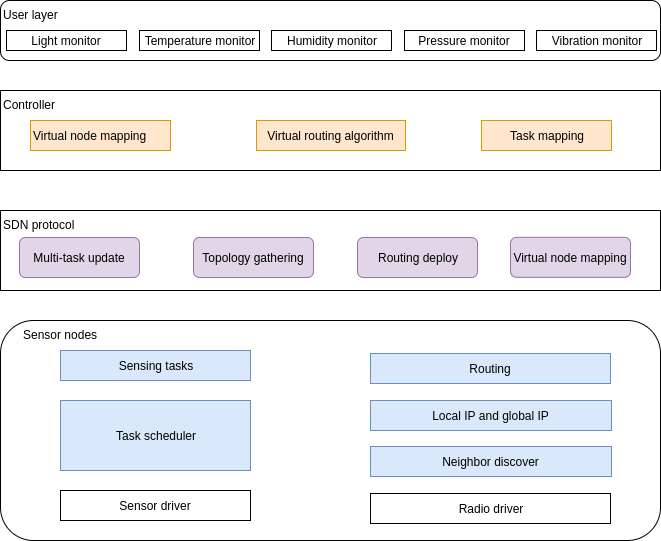
\includegraphics[width=3.5in]{./Figure/Architecture}
	\caption{Architecture of the system.}
	\label{Architecture}
\end{figure}

To build software defined network system in WSN and achieve low 
energy consumption and high performance, the SDN controller ought to  
configure data plane within as less hops as possible.  
In {\sdn}, we choose UAV as a mobile SDN controller,  
which communicates with sensor nodes by on-hop communication.
It significantly reduces the energy consumption of nodes in {\sdn}. 
To achieve high performance, the UAV controller carries
a powerful airborne computer which has ability to run 
some intelligent applications in real-time.

\subsection{SDN Planes}
The \textbf{data plane} runs on sensor nodes while the control 
plane and management plane run on UAV controller. 
And the interface between data plane and control plane is defined as a southbound interface,
while the interface between control plane and management plane is defined as a northbound interface.

In the \textbf{control plane}, in order to make our system easy to use,  we implement a database on the UAV and design interfaces for data plane and SDN applications. The control plane connected data plane and 
management plane. The database maintain the topology gathered from the data plane, route table inputed form applications, and sensor task schedule table form management application.

On \textbf{management plane}, user can run tons of applications base on our well-defined southbound APIs, such as routing algorithms, network diagnose, sensor task 
scheduler, etc.


Different from wired network, the data plane of WSN not only runs
data forwarding function, but also executes data sampling function. 
For example,  sensor nodes execute neighbor discovery process for getting topology, 
data sampling process for getting data from environment and data forwarding process
for data gathering. {\sdn} is an easy-to-use system that we design and implement a lot of 
interfaces for users.
\subsection{Southbound Data Structures}
As shown in Fig \ref{downstream} and Fig \ref{upstream}, the \textbf{southbound data structure} including downstream and upstream structure fully considered the difference between wired networks and wireless sensor networks, the data structure not only contains routing  related data, but also has sensor task control tables.

\begin{figure}[htbp]
	\centering
	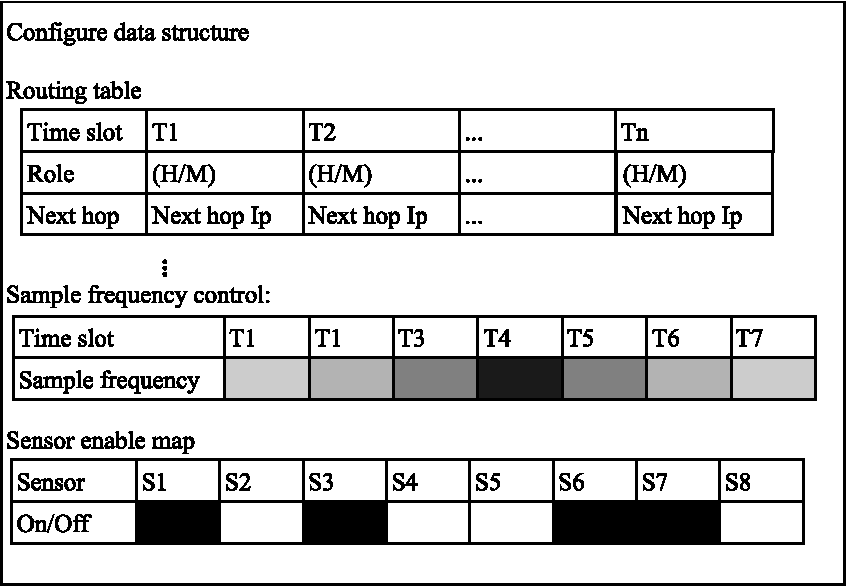
\includegraphics[width=1\columnwidth]{Figure/downstream}
	\caption{Downstream data structure}
	\label{downstream}
\end{figure}

\begin{figure}[htbp]
	\centering
	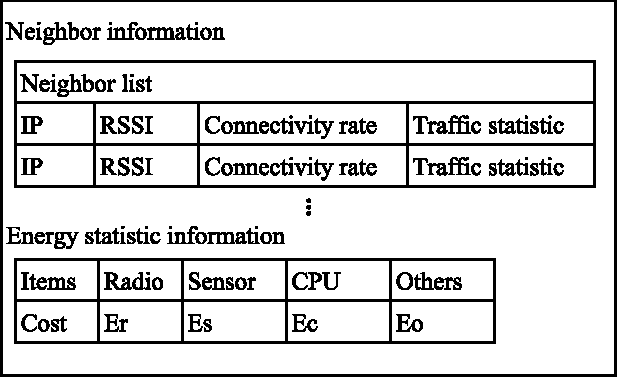
\includegraphics[width=1\columnwidth]{Figure/upstream}
	\caption{Upstream data structure}
	\label{upstream}
\end{figure}


\subsection{Southbound Interface}
The Table \ref{API} shows our southbound interface for user write applications. By using our SDN Southbound Interface, users can easily write 
a variety of applications, such as routing protocol, sensor task scheduler, network diagnose, algorithm evaluator, etc.
\begin{table*}[!t]
	\caption{SDN Southbound Interface}
	\label{API}
	\centering
	\scalebox{0.9}{
	\begin{tabular}{|l|l|}
		\hline
		\makecell[tc]{\textbf{Structure \&\& Function}} & \makecell[tc]{\textbf{Description}} \\
		\hline
		\multicolumn{2}{|c|}{\textbf{Sensor Control Interface}}\\
		\hline 
		\hline
		struct node & Sensor node structure\\
		\hline
		struct nodeset & A set of sensor nodes \\
		\hline
		struct neighbor\_list & Neighbor infomation \\
		\hline
		struct energy\_item & Energy statistic information \\
		\hline
		struct rout\_table & Route table \\
		\hline
		struct duty\_cycle\_table & Duty cycle control table \\
		\hline
		struct sensor\_enable\_table & All the nodes's states. Node state: \{on,off\} \\
		\hline
		switch\_node(node,state) & Turn on or turn off the node \\
		\hline
		get\_node\_info(node) & Get node's information, including  node's position, duty cycle, power, etc.\\
		\hline
		set\_node\_attr(node,attrTag,value) & Set node attribute, including  duty cycle, radio strength, etc. \\
		\hline
		get\_neighborlist(node) & Get the neighbor list of a node \\
		\hline
		\multicolumn{2}{|c|}{\textbf{UAV Application Interface}}\\
		\hline
		\multicolumn{2}{|c|}{\textbf{Routing}}\\
		\hline 
		\hline
		get\_topology() & Get the topology of the network\\
		\hline
		get\_rout\_table(node) & Get the route table of a node \\
		\hline
		set\_route(node) & Set the route of a node \\
		\hline
		\multicolumn{2}{|c|}{\textbf{AI Node selection}}\\
		\hline
		\hline
		nodeset simple\_selection(nodeset) & Select sensor set by location information\\
		\hline
		nodeset SRSSS\_selection(dataset) & Select sensor set by AI algorithm based on sensing data\\
		\hline
		\multicolumn{2}{|c|}{\textbf{AI Energy Prediction}}\\
		\hline
		\hline
		model\_selsct(modeltype) & Select an AI model\\
		\hline
		model.train(dataset,ratio) & Train an AI model with learning ratio on the data set\\
		\hline
		model.test(dataset) & Test the AI model on the data set\\
		\hline
		model.predict(node) & Do the energy prediction for a node \\
		\hline
		\multicolumn{2}{|c|}{\textbf{Multi-tasks}}\\
		\hline
		\hline
		create\_scheduler() & Create a task scheduler \\
		\hline
		scheduler.create\_buffer() & Create a task buffer \\
		\hline
		scheduler.task\_buffer\_add(task,nodeset) & Add a new task to task buffer \\
		\hline
		scheduler.task\_buffer\_remove(task) & Remove a new task to task buffer \\
		\hline
		scheduler.task\_buffer\_update(task,nodeset) & Update a task to task buffer with a new nodeset \\
		\hline
		scheduler.task\_update() & Schedule the added or removed tasks in the buffer\\
		\hline
		\multicolumn{2}{|c|}{\textbf{Diagnosis}}\\
		\hline
		\hline
		detect() & Detect problematic region with probes \\
		\hline
		get\_topical\_topology(nodeset) & Construct topical topology\\
		\hline
		diagnose\_network(topology,nodeset) & Diagnose the failure nodes or lossy links\\
		\hline
	\end{tabular}
	}
\end{table*}

We demonstrate two application code using our southbound interface. The List. \ref{topology-update} shows a deployed routing algorithm based on our SI. 
And the List. \ref{AI} demonstrate a AI selection and Muti-tasks application.

\begin{lstlisting}[
	language={[ANSI]C},
	label=topology-update,caption={An example of deploy routing algorithm},
	keywordstyle=\color{blue!70},
	showstringspaces=false,
	commentstyle=\color{red!50!green!80!blue!70},
	frame=single,captionpos=t,
	rulesepcolor=\color{red!20!green!20!blue!20},
	basicstyle=\ttfamily]
topology = get_topology();
//calculate route table for each node
//based on topology
for(node=0; node<nude_num; node++){
   node.routingtable =
      calculate_routable(topology);
}
//set route table for each node
for(node=0; node<nude_num; node++){
   fly_to(node);
        set_route(node.routingtable);
}

\end{lstlisting}

\begin{lstlisting}[language={[ANSI]C},label=AI,
	caption={An example of AI selection and Muti-tasks},
	keywordstyle=\color{blue!70},
	showstringspaces=false,
	commentstyle=\color{red!50!green!80!blue!70},
	frame=single,captionpos=t,
	rulesepcolor=\color{red!20!green!20!blue!20},
	basicstyle=\ttfamily]
AI_Multitasks(taskset){
   create_scheduler();
   scheduler.create_buffer();

   for(task=taskset.head; task < taskset.len;task=task.next)
      scheduler.task_buffer_add(
         task,
         defaultset);

   scheduler.task_update();
   ...
   ...
   while((task = scheduler.task_next)!= NULL){
      data = get_collected_data();
      nodeset =
         SRSSS_selection(dataset);
      scheduler.task_buffer_update(
         task,
         nodeset);
   }
   scheduler.task_update();
}

\end{lstlisting}

